\documentclass{webofc}
\usepackage[utf8]{inputenc}
\usepackage{graphicx}
\usepackage[varg]{txfonts}
\usepackage{subfigure}
\usepackage{appendix}

\title{Generative Models for Fast Calorimeter Simulation}
\subtitle{LHCb case}

\author{
 \firstname{Viktoria} \lastname{Chekalina} \inst{1,2}\fnsep\thanks{\email{sayankotor1@gmail.com}}
\and
    \firstname{Elena} \lastname{Orlova} \inst{3}\fnsep\thanks{\email{egorlova68@gmail.com}}
\and
    \firstname{Fedor} \lastname{Ratnikov} \inst{1,2}
\and
     \firstname{Dmitry} \lastname{Ulyanov} \inst{3}
\and
     \firstname{Andrey} \lastname{Ustyuzhanin} \inst{1,2}
\and
     \firstname{Egor} \lastname{Zakharov} \inst{3}\fnsep\thanks{\email{eo.zakharov@gmail.com}}
}

\institute{
NRU Higher School of Economics, Moscow, Russia
\and
Yandex School of Data Analysis, Moscow, Russia  
\and
Skolkovo Institute of Science and Technology, Moscow, Russia
}
        
\abstract{Simulation is a key component of high energy physics. Historically simulation in particle physics relies on the Monte Carlo methods which require a tremendous amount of computation. These methods may have difficulties with the expected High Luminosity Large Hadron Collider (HL LHC) need, so the experiment is in urgent need of new fast simulation techniques. We introduce a new Deep Learning framework based on Generative Adversarial Networks which can be faster than traditional simulation methods by 5 order of magnitude with reasonable simulation accuracy. This approach will allow physicists to produce a big enough amount of simulated data needed by the next HL LHC experiments using limited computing resources.}

\begin{document}

\maketitle

\section{Introduction}
Simulation is an important part of studies in particle and nuclear physics from the initial detector design phase to the final comparison with theoretical models. Traditionally, simulations rely on the Monte Carlo methods which require significant computational resources that will not scale to meet the growing demands resulting from large quantities of data expected during High Luminosity Large Hadron Collider (HL LHC) runs. One of the most well known examples of simulation software based on the Monte Carlo methods is \texttt{Geant4} \cite{agostinelli2003geant4} implementing cutting-edge heuristics and algorithms. The detailed simulation of particle collisions and interactions using \texttt{Geant4} as captured by detectors at the LHC annually requires billions of CPU hours constituting more than half of the LHC experiments' computing resources \cite{bozzi2014, flynn2015computing}. More specifically, the detailed simulation of particle showers in calorimeters is the most computationally demanding step.

% Other approaches which are based on using previously calculated or measured physical quantities have been applied in order to reduce the computation time \cite{grindhammer2000parameterized,atlas2010simulation}. This approach suffers from being specific to an individual experiment and despite being faster than full simulation it still takes relatively long to apply. Thus, the particle physics community is in need of new faster methods to model experiments. 
    
One of the possible approaches to simulate the calorimeter response is using the deep learning techniques. In particular, the Generative Adversarial Networks based approach has been applied sufficiently to the similar task of modeling particle showers in multi-layer Calorimeters with speed-up factors of up to 100 000 \cite{paganini2017calogan}. In our case, a particle is described by 5 parameters: 3d momentum $(p_x,~ p_y,~ p_z)$ and 2d coordinate $(x,~ y)$. We propose a new Deep Learning based framework for high-fidelity fast simulation of particle showers in the specific LHCb calorimeter in order to replace the existing Monte Carlo based methods and achieve a significant speed-up factor.

\section{Related work}
Generative models are of great interest in deep learning. These models can be utilized for natural looking pictures or video producing. In this section we give a brief overview of the most popular generative model in computer vision --- GANs, its strong and weak sides and different modifications to struggle with some issues. Also we analyze an article about applying GANs to the simulation problem in physics.

\subsection{Generative models}
GANs were originally presented by Goodfellow in 2014 \cite{goodfellow2014generative} and quickly became a state-of-the-art technique in areas such as image generation \cite{radford2015unsupervised}. The main idea of GAN can be described as follows.

We attempt to mimic a given target distribution $p_{\text{data}} (\textbf{x})$ by constructing two networks $\G$ and $\D$ called the generator and the discriminator. The generator learns to sample from the target distribution by transforming a random input vector $\textbf{z}$ to a vector $\textbf{x} = \G$ and the discriminator learns to distinguish the model distribution $p_\text{model} (\textbf{x})$ from $p_{\text{data}} (\textbf{x})$. The described procedure is presented in Fig. \ref{fig:GANs}.

\begin{figure}[h!]
\centering
\begin{tabular}{0.5\textwidth}
  \centering
  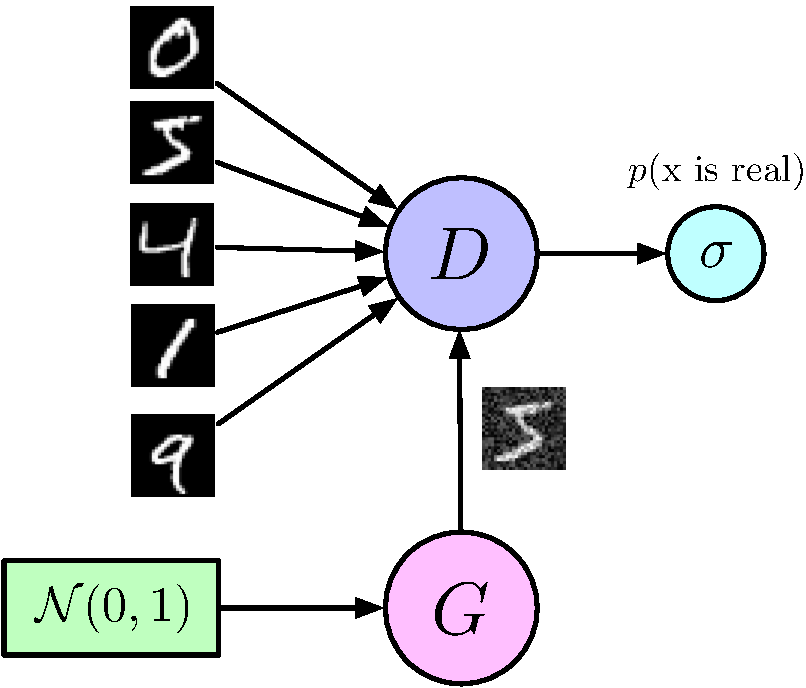
\includegraphics[width=0.3\linewidth]{figures/gan_pic.pdf}
\end{tabular}
\caption{Generative Adversarial Networks. There are two networks: the generator $G$ which transforms the noise vector to an image and the discriminator $D$ which classifies inputs as real or fake. We train them in adversarial manner, so, the task of $G$ is to make $D$ think that produced images are real. As the result, $G$ learns to reproduce the data distribution.}
\label{fig:GANs}
\end{figure}

The training procedure for GANs is typically based on applying gradient descent in turn to the discriminator and the generator in order to minimize a loss function which serves as a substitute to the exact formulation based on finding a Nash equilibrium in a non-convex game:
\begin{equation}\label{eq1}
\min_G \max_D \mathbb{E}_{\textbf{x} \sim p_{\text{data}}} [\log D(\textbf{x})] + \mathbb{E}_{\textbf{z} \sim p(\textbf{z})} [\log(1 - D(G(\textbf{z})))],
\end{equation}
where $\textbf{x} \sim p_{\text{data}}$ are samples from the input data, $\textbf{z} \sim p(\textbf{z})$ are the random noise samples, $G(\textbf{z})$ are the generated images and $D(G(\textbf{z}))$ is the output of the discriminator specifying the probability of an input being real.

In practice, this method ends up with generative neural nets that are considerably effective at producing new data. The main benefit of this approach is that GANs training procedure is easier in contrast with previous probabilistic models like Boltzmann machines.

\subsubsection{Wasserstein GAN}
There are various modifications of GANs for struggling with some typical problems and for improving the training procedure. A common GANs issue is so--called mode collapse when $p_\text{model} (\textbf{x})$ fails to capture a multimodal nature of $p_{\text{data}}(\textbf{x})$ and in extreme cases all the generated samples might be identical, in more involved architectures such as Waserstain GAN \cite{arjovsky2017wasserstein} the discriminator loss is argued to be consistent with the image quality. The main idea is to apply the Wasserstein-1 distance in order to compare $p_{\text{data}}$ and $p_{\text{model}}$.

Let $\mathbb{X}$ be a compact metric set and let $\mathbb{B}$ denote the set of all the Borel subsets of $\mathbb{X}$. Let $Prob(\mathbb{X})$ denote the space of probability measures defined on $\mathbb{X}$. The \emph{Earth-Mover} or \emph{Wasserstein-1} distance between two distributions $\mathbb{P}_r, \mathbb{P}_g \in Prob(\mathbb{X})$ is defined in the following way:

\begin{equation}\label{wasserstein_metric}
W(\mathbb{P}_r, \mathbb{P}_g) = \inf_{\gamma \in \Pi(\mathbb{P}_r, \mathbb{P}_g)} \mathbb{E}_{(x, y) \sim \gamma} \big{[}\|\textbf{x}-\textbf{y}\|\big{]},
\end{equation}

where $\Pi(\mathbb{P}_r, \mathbb{P}_g)$ is the set of all joint distributions $\gamma(x, y)$ whose marginals are respectively $\mathbb{P}_r$ and $\mathbb{P}_g$. $\gamma(x, y)$ denotes how much “mass” must be transported from $x$ to $y$ in order to transform the distributions $\mathbb{P}_r$ into the distribution $\mathbb{P}_g$. Thus, the Wasserstein distance can be defined as the minimum cost of transporting mass in order to transform the distribution $\mathbb{P}_r$ into the distribution $\mathbb{P}_q$. 

By applying to this distance the \emph{Kullback--Leibler divergence}, the \emph{Jensen-Shannon divergence} and the Kantorovich--Rubinstein duality and also parameterization of family of functions $\{f_w\}_{w \in \mathcal{W}}$ that are all K-Lipschitz for some K we could consider solving the problem (for more detailed information see the paper \cite{arjovsky2017wasserstein})

\begin{equation}\label{optim}
\max_{w \in \mathcal{W}} \mathbb{E}_{x \sim P_r}[f_w(x)] - \mathbb{E}_{z\sim p(z)} [f_w(g_\theta(z))]
\end{equation}

and if the supremum in \eqref{optim} is attained for some $w \in \mathcal{W}$, this process would lead to a calculation of $W(\mathbb{P}_r, \mathbb{P}_\theta)$ up to a multiplicative constant.
So, the WGAN value function is
\begin{equation}\label{wgan_loss}
\min_G \max_{D \in \mathcal{D}}  \mathbb{E}_{\textbf{x} \sim \mathbb{P}_r}  [D(\textbf{x})] - \mathbb{E}_{\tilde{\textbf{x}} \sim \mathbb{P}_g} [D(\tilde{\textbf{x}})],
\end{equation}
where $\mathcal{D}$ is the set of 1-Lipschitz functions and $\mathbb{P}_g$ is  the model distribution defined by $\tilde{\textbf{x}} = G(\textbf{z}), ~\textbf{z} \sim p(\textbf{z}).$

In general, the training procedure of GANs is known to be difficult and presents such issues as mode collapse, and WGAN often helps to overcome this problem.

The Wasserstein GAN value function makes optimization process easier because the discriminator's gradient with respect to its input is better behaved than its GAN counterpart. Also, it was noticed that the WGAN value function tend to correlate with the original data quality which is not always the case for ordinary GANs.


\subsubsection{Wasserstain GAN with gradient penalty}
An alternative way to enforce the Lipschitz constraint was introduced in \cite{gulrajani2017improved}. The authors consider directly constraining the gradient norm of the discriminator$\textquotesingle$s output with respect to its input because a differentiable function is 1-Lipschtiz if and only if it has gradients with norm at most 1 everywhere. To come over tractability issues a soft version of the constraint with a penalty on the gradient norm for random samples $\tilde{\textbf{x}} \sim \mathbb{P}_{\tilde{\textbf{x}}}$ was suggested. Therefore, a new obtained objective is 
\begin{equation} \label{gpwgan-loss}
\begin{gathered}
\mathcal{L}(\bm{\theta}) =
\underbrace{ \underset{\tilde{\textbf{x}} \sim \mathbb{P}_g}{\mathbb{E}}  \Big[D(\tilde{\textbf{x}})\Big] - \underset{\textbf{x} \sim \mathbb{P}_r}{\mathbb{E}} \Big[D(\textbf{x})\Big]}_{\text{original loss}} + 
\underbrace{ \lambda \underset{\textbf{x} \sim \mathbb{P}_g}{\mathbb{E}} \Big[\big(\|\nabla_{\tilde{\textbf{x}}} D(\tilde{\textbf{x}})\|_2 - 1\big)^2 \Big]}_{\text{gradient penalty}}.
\end{gathered}
\end{equation}

This approach demonstrates strong modeling performance and stability across a variety of architectures.  Now it is a state-of-the-art technique in GANs. 
How to calculate this loss in practice is described on Sec. \ref{training_strategy}.

\subsection{GANs in high energy physics}
The first systematic study on the application of Deep Learning to Particle Physics was carried out by Paganini et al. in 2017. In the paper \cite{paganini2017calogan} the authors investigated application of GANs for detailed particle simulation in the 3-layer unheterogeneous calorimeter at the LHC. \texttt{Geant4} was utilized to create the dataset. Positrons, photons and charged pions with various energies are incident perpendicular on the center of the calorimeter front. Energies in the training are uniform in the range between 1 GeV and 100 GeV.  The first layer was represented as a $3 \times 96$ image, the middle layer as a $12 \times 12$ image, and the last layer as a $12 \times 6$ image. 

The implemented model is called CaloGAN and the main architecture feature is using the locally-connected layers \cite{taigman2014deepface} to modify DCGAN structure \cite{radford2015unsupervised}. The idea of locally connected layers is based on the fact that every pixel position gets its own filter while an ordinary convolutional layer has a set of  same parameters for every position. Spreading of this method to particle physiscs simulation was described in the previous work of the authors and such type of neural network was called LAGAN \cite{de2017learning}. A special section in the paper is devoted to the evaluation of the quality of the CaloGAN produced images where  sparsity level,  energy per layer or total energy are suggested to measure the performance of the model. 

The obtained results demonstrate a prospect of application of GANs for the particle showers generation and replacing of the Monte Carlo methods with the proposed approach. The CaloGAN shows sizable simulation-time speed ups compared to \texttt{Geant4}. 

In fact, the CaloGan model is based on DCGAN with the described tricks. However, GANs tend to suffer from mode collapse. Therefore, the CaloGan architecture cannot be applied for all datasets, because there is a high probability of mode collapse appearance and it is a limitation of this work.

\section{Our model} \label{sec:model}
Our idea is to treat simulations as a black-box and replace the traditional Monte Carlo simulation with a method based on Generative Adversarial Networks. WGANs with gradient penalty are considered to be state-of-the-art technique for image producing, so we decide to implement a tool based on this particular approach. For it to be useful in realistic physics applications such a system needs to be able to accept requests for the generation of showers originating from an incoming particle parameters such as 3d momentum and 2d coordinate. We introduce an auxiliary task of energy reconstruction to condition on these parameters $p_x$, $p_y$, $p_z$ and $x$, $y$.

\subsection{Dataset}
At the work we focused on electrons interactions inside the electromagnetic calorimeter at the LHCb. In particular, the calorimeter used in this study employs "shashlik" technology of alternating scintillating tiles and lead plates. It consists of 5 $\times$ 5 blocks of size 12 cm $\times$ 12 cm, the cell granularity corresponds to each block is 5 $\times$ 5 of size 2 cm $\times$ 2 cm. There are 66 layers in ECAL -- 2 mm absorber and 4 mm scintillator. In fact, the shower appears in 3d, but we summarized allocated energies in each layer per cell. This procedure does not obstruct physics analysis and does not inhibit the shower shape. Thus, this information can be represented as 30 $\times$ 30 images $Y$ with the corresponding parameters $(p_x,~ p_y,~ p_z,~ x,~ y)$. Such image example is presented in \ref{fig:real-imgs}.

The training data set is created as follows. \texttt{Geant4} is utilized to generate particles and simulate their interaction with the calorimeter using the \texttt{Ftfp\_Bert} physics library based on the \texttt{Fritiof}  and \texttt{Bertini} intra-nuclear cascade models with the standard electromagnetic physics package. So information about every event includes the parameters and 30 $\times$ 30 matrix of energies deposited in scintillator for every cell tower $Y$. Size of the training dataset is 50 000 events, and we have 10 000 events at the test dataset.

\subsection{Model architecture}

We need to generate a specific calorimeter response to a particle with some parameters. It means that a model is required to be conditional.
% sampling not just from $p(\textbf{y}),$ but from $p(\textbf{y}|\textbf{x}),$ so, 
Firstly, we describe a generator and discriminator architecture. The generator maps from an input (a 512 $\times$ 1 vector sampled from the Gaussian distribution and the particle parameters) to an 30 $\times$ 30 image $\hat{\textbf{y}}$ using deconvolutional layers (in fact, it is an upsampling procedure and convolutions) which are arranged as follows. We concatenate the noise vector and the parameters $(p_x,~ p_y,~ p_z,~ x,~ y)$, after that we add a fully connected layer with reshaping and obtain 256 $\times$ 4 $\times$ 4 output. After a sequence of 2d deconvolutions we get outputs of size  128 $\times$ 8 $\times$ 8, 64 $\times$ 15 $\times$ 16 and 32 $\times$ 32 $\times$ 32  with ReLu activation functions. After this procedure we crop the last output to obtain the image of desired size 30 $\times$ 30.

As for the discriminator, it takes a batch of images as input (all images in the batch are real or generated by $G$) and returns the score $D(\textbf{y})$ or $D(\hat{\textbf{y}})$ as it is described in \cite{arjovsky2017wasserstein}. Discriminator architecture is simply the reversed generator architecture (i.e. sizes of layers go in the opposite order). It implies that we have 30 $\times$ 30 matrix as input, then we obtain layers outputs of size 32 $\times$ 32 $\times$ 32, 64 $\times$ 15 $\times$ 16, 128 $\times$ 8 $\times$  8, after that reshaping leads to 256 $\times$ 4 $\times$ 4, and by applying LeakyRelu activation function we get the final score. The model scheme is presented in Fig. \ref{fig2:model}.

\begin{figure}[h!]
\centering
\begin{subfigure}
  \centering
  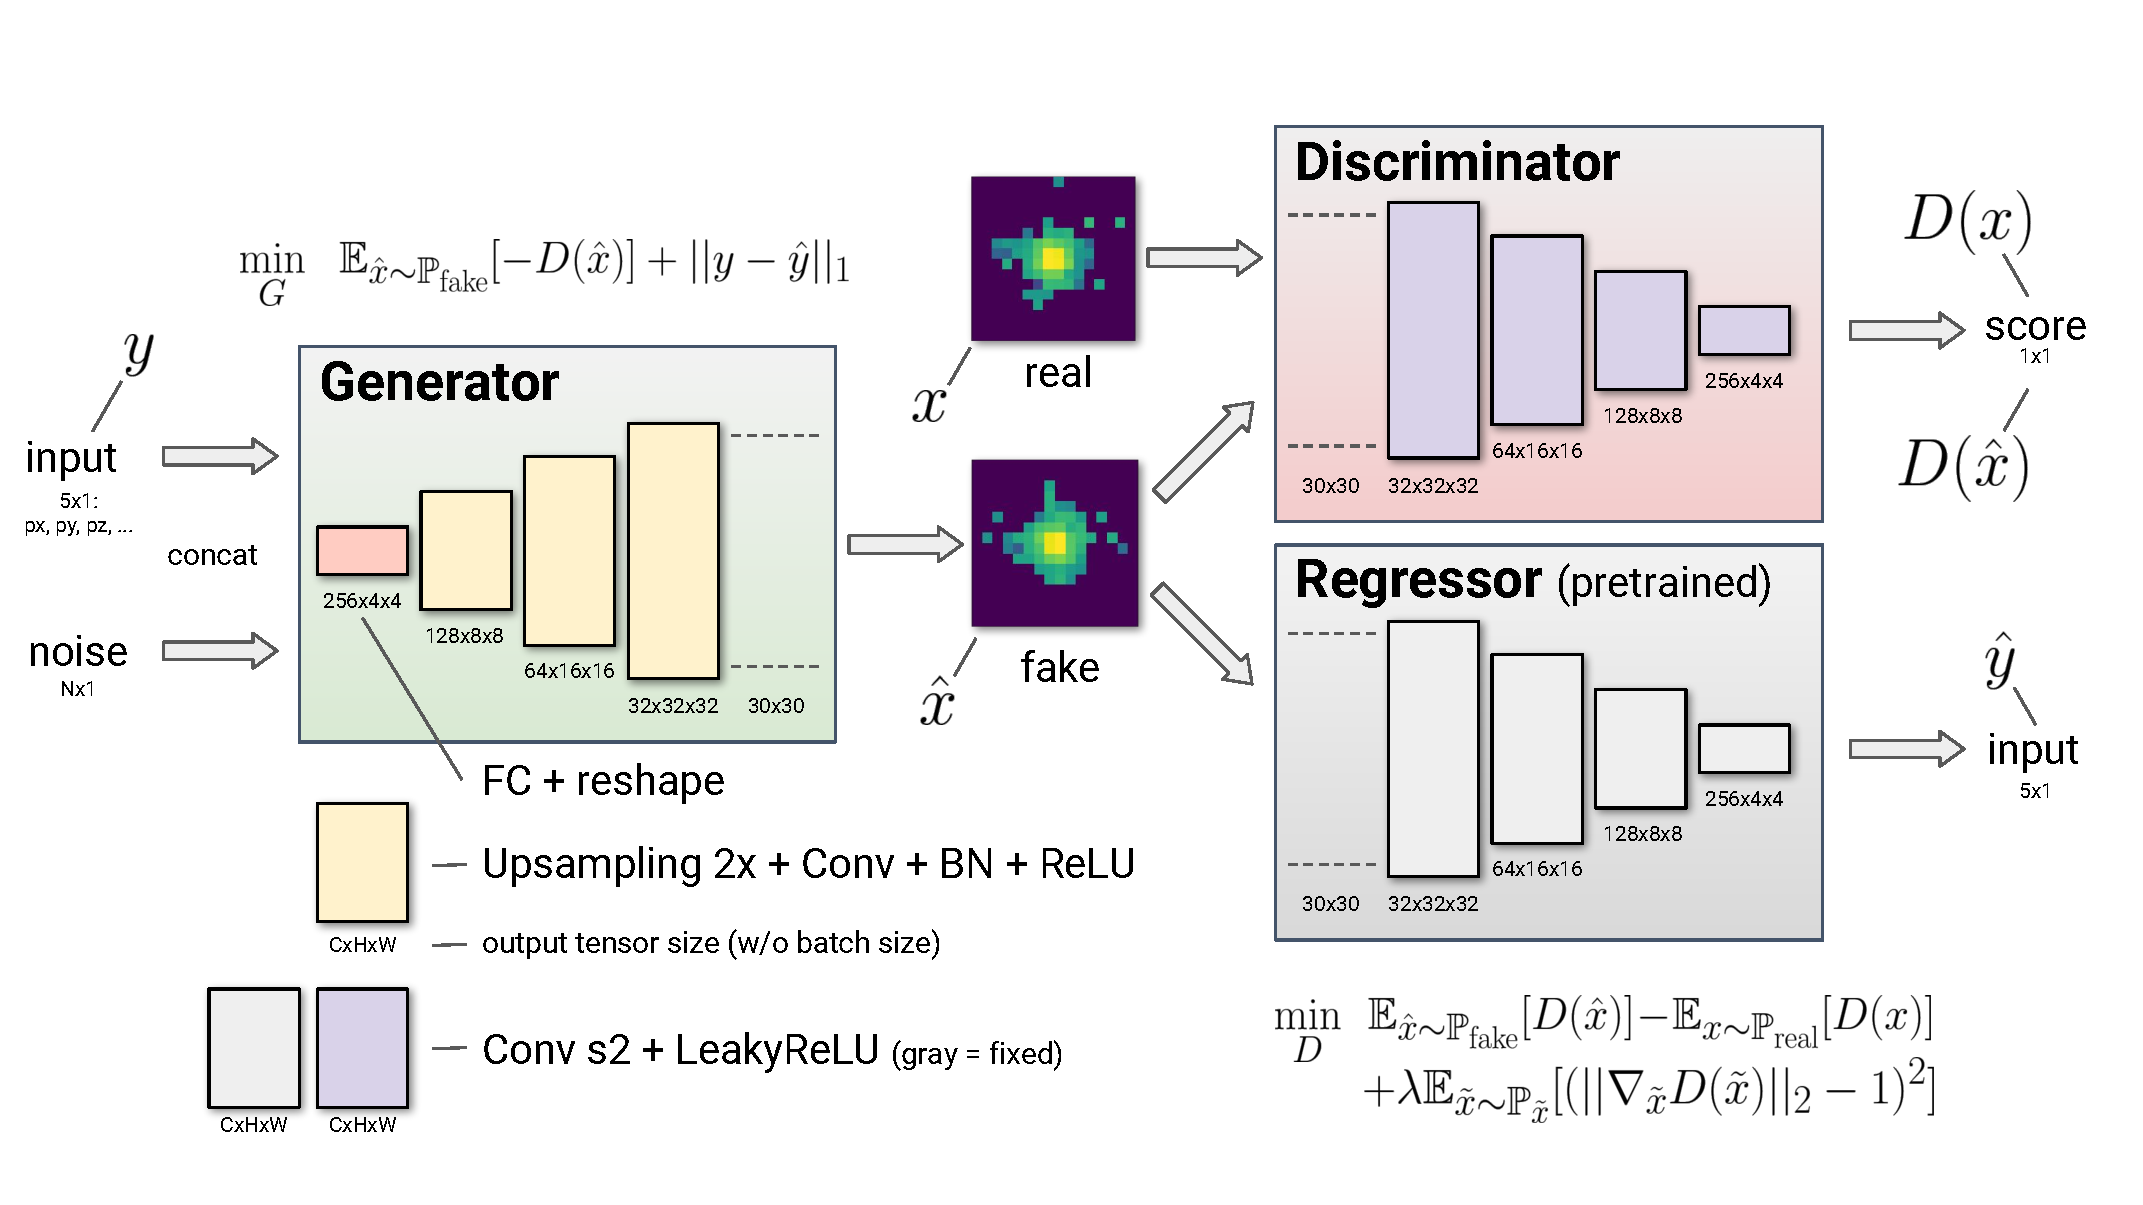
\includegraphics[width=0.7\linewidth]{figures/model_architecture.pdf}
\end{subfigure}%
\caption{Model architecture. Pretrained regressor for the particle parameters prediction makes our model conditional. Thanks to building up the information from the pretrained regressor into the discriminator gradient we learn $G$ to produce a specific calorimeter response.}
\label{fig2:model}
\end{figure}

How to train WGAN with gradient penalty in conditional manner is described in the following section.

\subsection{Training strategy} \label{training_strategy}
Due to the nature of WGAN loss, conditioning on the continuous value is a non-trivial task. To overcome this issue we suggest to embed a pretrained regressor in our model. We train a neural network to predict the particle parameters by the calorimeter response. As for architecture, it has the same one as the discriminator but with a perceptual loss described in \cite{johnson2016perceptual} because, as we figured out, it works better rather than standard MSE. By building up the information from the pretrained regressor into the discriminator gradient, we obtain the conditional model because we train the generator and the discriminator together. Now the discriminator makes the generator produce a specific calorimeter response.

Matrices from our dataset are pretty sparse because almost all information is located in central cells (see in Fig. \ref{fig:real-imgs}). To make optimization process easier we apply a box--cox transformation. This mapping helps to smooth the data that makes the optimization process more stable.
Results obtained with the described model are presented in the following section.

\section{Results}
From a series of simulated electron showers our conditional GAN is tasked with learning the simulated data distributions generated by \texttt{Geant4}. There exist several methods to estimate the performance of generative models, but not all evaluation criteria are equally suitable and reliable for all applications. In our paper we focus on quantitative evaluation based on physics-driven similarity metrics. The choice reflects the domain specific procedure for data-simulation comparison. 

Examples of real and produced images are presented in Fig.b\ref{fig:gen-img}. It can be concluded that produced images look quite similar to the original data but we are also supposed to do more deep analysis.



\begin{figure}[h]
  \centering
  \subfigure[E = 63.7~ $\text{GeV}$ \\ \centering $\frac{p_x}{p_z}$=0.005 $\frac{p_y}{p_z}$=0.154]{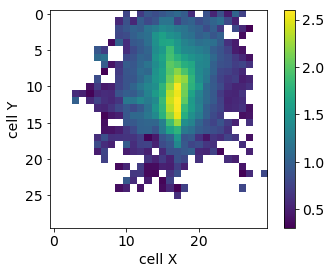
\includegraphics[width=0.2\textwidth]{figures/1_real.png}}
  \subfigure[E = 6.5~ $\text{GeV}$ \\ \centering $\frac{p_x}{p_z}$=0.046~ $\frac{p_y}{p_z}$ = 0.108]{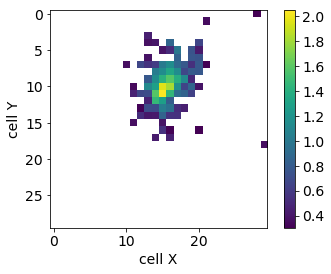
\includegraphics[width=0.2\textwidth]{figures/2_real.png}}
  \subfigure[E = 15.6 $\text{GeV}$ \\ $\frac{p_x}{p_z}$=-0.196 $\frac{p_y}{p_z}$=- 0.036]{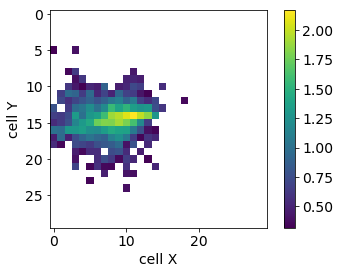
\includegraphics[width=0.21\textwidth]{figures/3_real.png}}
  \subfigure[E = 15.6 $\text{GeV}$ \\ $\frac{p_x}{p_z}$=-0.019$\frac{p_y}{p_z}$=0.181]{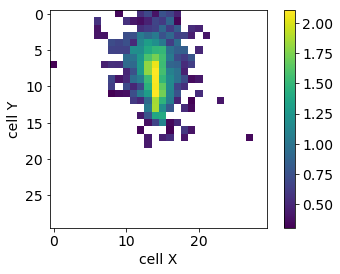
\includegraphics[width=0.21\textwidth]{figures/4_real.png}} 
  \caption{Images and the parameters from the real dataset.}
  \label{fig:real-imgs}
\end{figure}

\begin{figure}[h]
  \centering
  \subfigure[E = 63.7~ \text{GeV} \\ \centering $\frac{p_x}{p_z}$= 0.005 $\frac{p_y}{p_z}$ = 0.154]{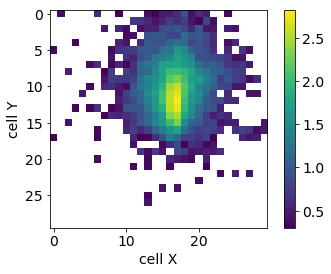
\includegraphics[width=0.2\textwidth]{figures/1_gen.png}}
  \subfigure[E = 6.5~ \text{GeV} \\ \centering $\frac{p_x}{p_z}$= 0.046~ $\frac{p_y}{p_z}$ = 0.108]{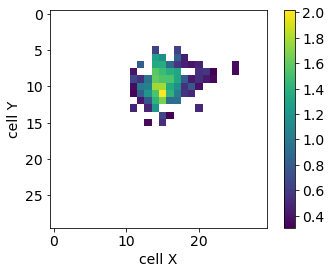
\includegraphics[width=0.2\textwidth]{figures/2_gen.png}}
  \subfigure[E = 15.6 Gev \\ $\frac{p_x}{p_z}$ = -0.196 $\frac{p_y}{p_z}$ = - 0.036]{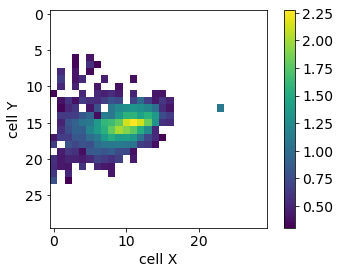
\includegraphics[width=0.21\textwidth]{figures/3_gen.png}}
  \subfigure[E = 15.6 GeV \\ $\frac{p_x}{p_z}$ = -0.019 $\frac{p_y}{p_z}$ = 0.181]{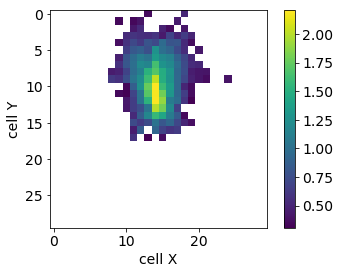
\includegraphics[width=0.2\textwidth]{figures/4_gen.png}}
  \caption{Images generated as a response to the parameters described in Fig. \ref{fig:real-imgs} inputted to the generator $G$. }
  \label{fig:gen-img}
\end{figure}

As a part of the analyzing generated images quality we calculated some physical characteristics of shower shapes such as cluster asymmetry, shower width and sparsity level. The obtained characteristics are presented in Fig. \ref{fig:quality}. How to calculate these variables is described in Appendix.

\begin{figure}[h]
  \centering
  \subfigure[The transverse asymmetry of real and generated images]{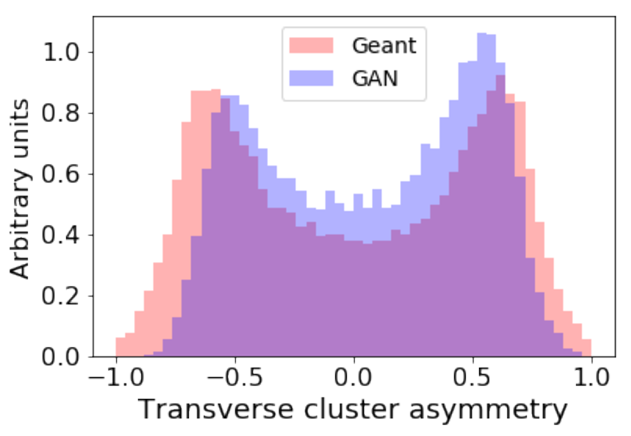
\includegraphics[width=0.3\textwidth]{figures/transverseAsymmetry.pdf}}
  \subfigure[The longitudal asymmetry of real and generated images]{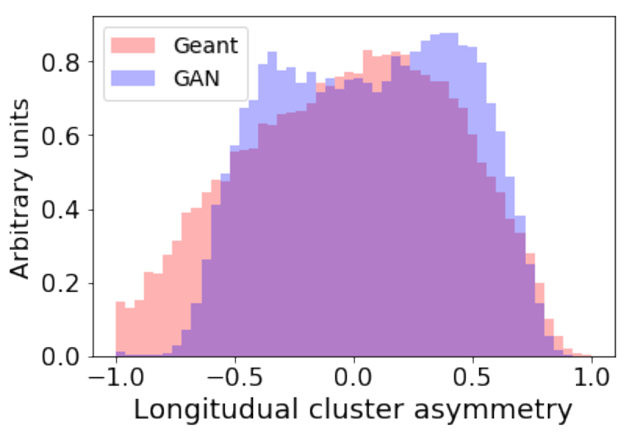
\includegraphics[width=0.3\textwidth]{figures/longAsymmetry.pdf}}
  \subfigure[The transverse width of real and generated images]{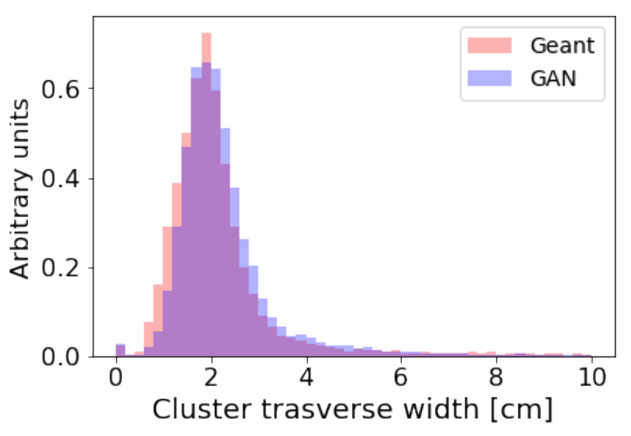
\includegraphics[width=0.3\textwidth]{figures/width.pdf}} 
  \subfigure[Delta X]{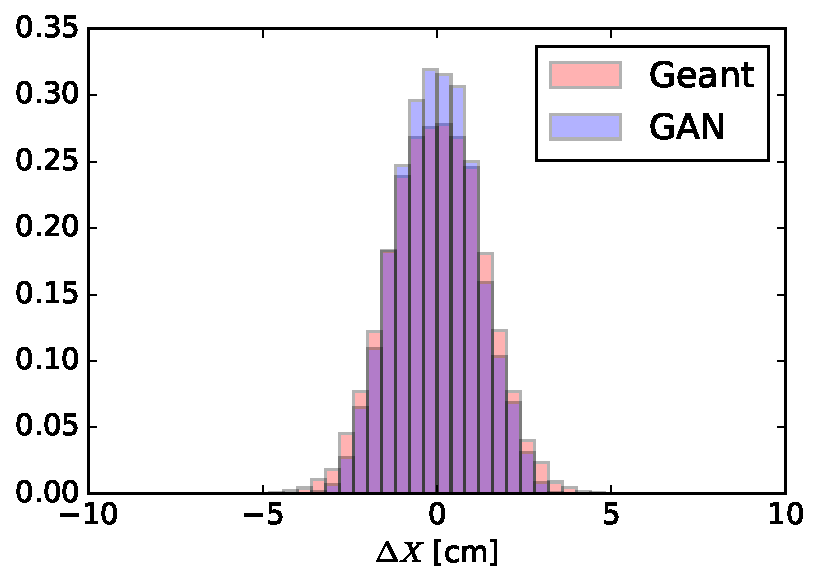
\includegraphics[width=0.3\textwidth]{figures/deltaX.pdf}}
  \subfigure[The sparsity of real and generated images]{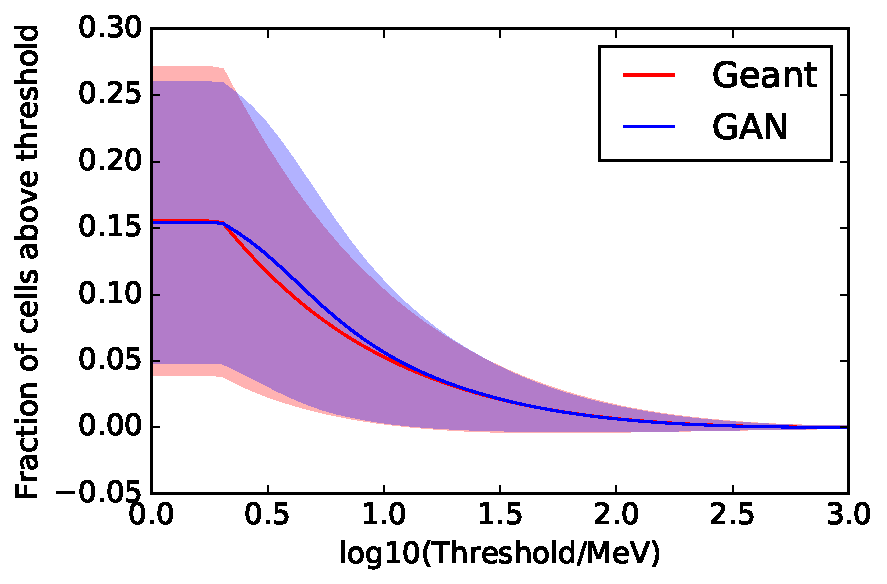
\includegraphics[width=0.3\textwidth]{figures/sparsity.pdf}}
  \caption{Generated images quality evaluation including described physical characteristics.}
  \label{fig:quality}
\end{figure}

The results are in good agreement with fully simulated data. Energy showers are faithfully reproduced and show a reasonable agreement with the standard Monte Carlo techniques. A detailed study to asses the quality of the GAN images using typical high level calorimeter reconstruction variables confirms this statement.

As for model performance, we trained our model for 3000 epochs which takes about 70 hours on GPU NVIDIA Tesla K80. The sampling rate is 0.07 ms per sample on GPU, 4.9 ms per sample on CPU.

\section{Conclusion and future outlook}\label{conclusion}
The research proves that Generative Adversarial Networks are a good candidate for fast simulating of high granularity detectors typically studied for the next generation accelerators. We have successfully generated images of shower energy deposition with a condition on the particle parameters such as the momentum and the coordinate using modern generative deep neural network techniques such as Wasserstain GAN with gradient penalty.

Future work will be focused improving obtained results such as shower shape characteristics.

\bibliography{main}
\bibliographystyle{plain}

\appendix
hello

\end{document}
